\documentclass[usegeometry=true]{scrartcl}
\usepackage[ngerman]{babel}
\usepackage[T1]{fontenc}
\usepackage{lmodern}
\usepackage[utf8]{inputenc}
\usepackage{hyperref}
\usepackage{amssymb}
\usepackage{csquotes}
\usepackage{graphicx}
\usepackage[table,xcdraw]{xcolor}
\usepackage[left=2cm, right=2cm, top=2cm, bottom=2cm, bindingoffset=1cm, includeheadfoot]{geometry}

\definecolor{codegreen}{rgb}{0,0.6,0}
\definecolor{codegray}{rgb}{0.5,0.5,0.5}
\definecolor{codepurple}{rgb}{0.58,0,0.82}
\definecolor{backcolour}{rgb}{0.95,0.95,0.95}


%--- Test
\usepackage{mdframed}
\usepackage{minted}


%Zeilenabstand bitte nicht ändern
\usepackage[onehalfspacing]{setspace}
\setlength{\parindent}{0em}
\usepackage[backend=biber,style=numeric,]{biblatex}\addbibresource{literatur.bib}

\begin{document}
% ----------------------------------------------------------------------------
\subject{Projektbericht zum Modul Information Retrieval und Visualisierung Sommersemester 2022}
\title{World Happiness Report 2021}
%\subtitle{Untertitel}% optional
\author{Johannes Boldt Matr.Nr.:}% obligatorisch
\date{}
\maketitle% verwendet die zuvor gemachte Angaben zur Gestaltung eines Titels
\pagenumbering{gobble}
% ----------------------------------------------------------------------------
\clearpage


% Inhaltsverzeichnis:
\tableofcontents
\clearpage
% ----------------------------------------------------------------------------
% Gliederung und Text:
\pagenumbering{arabic}

\section{Einleitung}

Zufriedenheit und Glück sind Themen die in der Forschung mehr und mehr an Bedeutung gewinnen. [Quelle]
Wie lassen sich diese Erfahrungen oder Emotionen überhaupt quantifizieren. Der World Happiness ist wohl eines der Umfassensten Forschungsprojekte welches sich mit diesem Thema und dem Glück auf der Welt am ausführlichsten Auseinandersetzt. Die Forscher erstellen jedes Jahr einen umfassenden bericht über alle Länder über die sie Daten erfassen können und stellen ein Happiness-ranking auf, also wie glücklich und zufrieden die verschiedenen Länder im jeweiligen Jahr sind. Diese Daten bilden die Grundlage dieser Arbeit. \\

In den letzten Jahren hat sich die Lebenszufriedenheit in vielen Teilen der Welt verbessert, insbesondere aufgrund der wirtschaftlichen Entwicklung und der Fortschritte in der Medizin und im Bildungswesen. Gleichzeitig gibt es jedoch auch viele Herausforderungen, die Lebenszufriedenheit beeinträchtigen können, wie zum Beispiel Arbeitslosigkeit, Armut, gesundheitliche Probleme und soziale Isolation. Gerade durch die COVID-19 Pandemie wurden viele Länder und deren Lebensqualität und Zufriedenheit beeinträchtigt. Auch damit beschäftigt sich der World Happiness Report 2021.  [quelle] \\

Eine visuelle Aufbereitung des World Happiness Reports könnte für eine Vielzahl von Personen und Organisationen von Nutzen sein, die an den Faktoren interessiert sind, die die Lebenszufriedenheit in verschiedenen Ländern beeinflussen. Dazu könnten zum Beispiel Regierungen, Unternehmen, Nichtregierungsorganisationen, Wissenschaftler, Journalisten und interessierte Bürger gehören. \\

Da der Bericht selber eine sehr ausführliche Beschreibung und Diskussion der Daten bietet, ist es Ziel dieser Arbeit einen schnelleren und intuitiven Zugriff auf die Daten und die enthaltenen Informationen zu bieten. Dabei sollen sich die Nutzer folgende Fragen mit den interaktiven Visualisierungen beantworten können. \\

\begin{itemize}
    \item Wie Zufrieden sind die Länder im Vergleich zueinander?
    \item Sind Zusammenhänge (Korrelation) zu erkennen zwischen der Zufriedenheit und erhobenen Variablen?
    \item Wie konstant sind die Werte über die letzen 10-20 Jahre. Entwickeln sich Länder stetig weiter oder machen einige auch Rückschritte?
\end{itemize}

\subsection{Anwendungshintergrund}
Das Gebiet der Lebenszufriedenheit ist ein wichtiger Bereich der Psychologie und Sozialwissenschaften, der sich mit dem subjektiven Empfinden von Glück, Zufriedenheit und Wohlbefinden befasst. Die Lebenszufriedenheit wird oft als ein wichtiger Indikator für das allgemeine Wohlbefinden und die Qualität des Lebens betrachtet, da sie mit einer Vielzahl von positiven Größen wie besserer Gesundheit, längerer Lebenserwartung und höherer Leistungsfähigkeit in Beziehung gebracht wird.
\\

Es gibt viele Faktoren, die die Lebenszufriedenheit beeinflussen, wie zum Beispiel persönliche Eigenschaften, soziale Beziehungen, Einkommen, Gesundheit, Umgebung und Lebensstil. Diese Faktoren können interagieren und sich gegenseitig beeinflussen, wodurch die Lebenszufriedenheit komplex und dynamisch ist.
\\

Der World Happiness Report beschäftigt sich seit Jahren instensiv mit diesem Thema. Diese jährlich veröffentlichte Studie wird von der United Nations Sustainable Development Solutions Network (SDSN) erstellt und bewertet die Lebenszufriedenheit in verschiedenen Ländern auf der Grundlage von Daten, die aus verschiedenen Quellen stammen, einschließlich Umfragen und Statistiken zu verschiedenen Indikatoren wie Einkommen, Gesundheit, Arbeitsbedingungen und sozialem Zusammenhalt. Der World Happiness Report bietet eine umfassende Perspektive auf die Lebenszufriedenheit auf globaler Ebene und kann dazu beitragen, das Verständnis der Faktoren, die die Lebenszufriedenheit beeinflussen, zu vertiefen und Maßnahmen zur Verbesserung der Lebenszufriedenheit zu identifizieren. 


\subsection{Zielgruppen}

Die Zielgruppe dieser Arbeit sind alle Personen die sich für Lebenszufriedenheit in der Welt interessieren, ausgenommen solcher die hierzu selber Forschung betreiben. Von viel Vorwissen ist daher nicht auszugehen. Daher müssen die Visualisierungen klar vermitteln können was dargestellt wird. Komplexe Darstellungen sind nicht angebracht. \\
Die Personen dieser Gruppe möchten mehr über Lebenszufriedenheit in der Welt erfahren und sich einen Eindurck vermitteln lassen wie diese verteilt ist. Diese Bedürfnisse sollen die Visualisierungen bedienen. 

\subsection{Überblick und Beiträge}
Die durch die Visualisierungen dargestellten Daten sind zweigeteilt. Die Durchschnitte der Jahre 2018-2020 sind die Basis aller Visualisierungen die keine Zeitliche Komponente enthalten. Sie sollen einen Ist-Zustand darstellen. Der zweite Datensatz sind die historischen Daten, diese bilden die Grundlage für die Zeitreihen Darstellung. \\

Die drei verwendeten Visualisierungen tragen unterschiedlich zu der Beantwortung der Nutzerfragen bei und vereinfachen allgemein die Zugönglichkeit der Daten. Der Scatterplot ermöglicht es Variablen und deren Korrelation übersichtlich darzustellen, zudem lassen sich hier Muster innerhalb von Ländergruppen identifizieren, da die Länder in Gruppen unterteilt und entsprechend Farblich hervorgehoben wurden. \\

Die zweite Visualisierung, der Polarplot gibt einen überblickt über die Variablen für ein Land. man gewinnt auf einem Blick einen Eindruck dafür wie ein Land aufgestellt ist in den verschiedenen Bereichen. Die letzte Visualisierung ist eine Zeitreihe mit leicht anderen gegebenen Variablen deren Erfassung teils bis zum Jahr 2006 zurückreichen. Hier lässt sich die Entwicklung von zwei Ländern gleichzeitig übersichtlich betrachten und vergleichen.

\section{Daten}

Die verwendeten Daten sind aus dem Kaggle-Datensatz \textit{World Happiness Report 2021}, die enthaltenen Daten wurden durch den World Happiness Report erfasst. Ajaypal Singh, der Ersteller des Kaggle Datensatzes hat keine Veränderungen an den gegebenen Daten vorgenommen, das Format wurde nur zu \textit{.csv} geändert. Man erhält die gleichen Daten wenn man sie von der \textit{World Happiness Report 2021} Seite herunterlädt. \cite{helliwell_world_2021}  \\

Die bereitgestellten Daten beeinhalten zwei separate Datensätze. Einen Datensatz mit historischen Daten, die für manche Länder bis 2005 zurückreichen, mit 9 gemessenen Größen für jedes Jahr. Und einen Datensatz der einen Vergleich der Länder für den Zeitraum 2018 - 2020 erstellt mit zusätzlichen Größen. Diese sind die ausgerechneten Faktoren für die gemessenen Größen und wie viel stark diese die Zufriedenheit in dem jeweiligen Land beeinflussen. \\

\begin{table}[h]
\centering
\resizebox{\textwidth}{!}{%
\begin{tabular}{|l|l|}
\hline
\rowcolor[HTML]{EFEFEF} 
Spaltenname &
  Beschreibung \\ \hline
Country name &
  Name des Landes \\ \hline
Regional indicator &
  Region zu welcher das Land gehört \\ \hline
Ladder score &
  \begin{tabular}[c]{@{}l@{}}Der Zufriedenheits Wert.\end{tabular} \\ \hline
Logged GDP per capita &
  Log umgewandeltes Bruttoinslandseinkommen pro Kopf \\ \hline
Social support &
  \begin{tabular}[c]{@{}l@{}}Nationaler Durchschnitt auf die Binäre Frage: {[}If you\\ were in trouble, do you have relatives or friends you can count on to help you\\ whenever you need them, or not?{]}\end{tabular} \\ \hline
Healthy life expectancy &
  Daten von der WHO über die gesunde Lebenserwartung im Land. \\ \hline
Freedom to make life choices &
  \begin{tabular}[c]{@{}l@{}}Nationaler Durchschnitt auf die Frage: {[}Are you satisfied or dissatisfied \\
    with your freedom to choose what you do with your life?{]} \end{tabular}\\ \hline
Generosity &
  \begin{tabular}[c]{@{}l@{}}Nationaler Durchschnitt auf die Frage, {[}Have you donated money to a charity in the \\ past month?{]}, regressiert auf das Bruttoinlandsprodukt pro Kopf\end{tabular} \\ 
\hline 
Perceptions of corruption &
  \begin{tabular}[c]{@{}l@{}}Nationaler Durchschnitt auf die Fragen: {[}Is corruption widespread throughout\\ the government or not{]} und {[}Is corruption widespread within businesses or not?{]}\end{tabular} \\ \hline
\end{tabular}%
}
\caption{Größen aus dem ersten Datensatz.}
\label{Tab:dat_1}
\end{table}

Tabelle \ref{Tab:dat_1} enthält die Größen des ersten Datensatzes und deren grobe Beschreibungen. Der \textit{Ladder Score} ist der Zufriedenheitswert oder Happiness Score. Der Kernwert des World Happiness Reports. Er wird \textit{Ladder Score} genannt aufgrund der Frage mit der er in Umfragen erfasst wird. Diese lautet unübersetzt: \textit{Please imagine a ladder, with steps numbered from 0 at the
bottom to 10 at the top. The top of the ladder represents the best possible life
for you and the bottom of the ladder represents the worst possible life for you.
On which step of the ladder would you say you personally feel you stand at this
time?"} \cite{helliwell_world_2021}. Der nationale Durchschnitt aus Antworten auf dies Frage bildet dann den Happiness Score. \\

Allerdings wurden einiger Variablen weggelassen. Jede der Variablen nach \textit{Ladder score} hatte eine weiter Instanz mit einer statischen Verechnung dieser um eine \textit{Explained by} Größe zu bilden. Diese stellen dar wie stark diese Größe wohl den erreichten Ladder Score erklärt. Da diese Variablen eher komplex sind und bereits im \textit{World Happiness Report}  ausführlich dargestellt werden, wurden sie nicht verwendet. Die verwendeten Fragen für die Variablenerfassung wurden nicht aus dem Englischen Übersetzt um deren Bedeutung nicht zu verzerren. Weiter Statistische Größen die ausgelassen wurden, sind der \textit{Standard Error}, \textit{lower whisker} und \textit{upper whisker}. \\

Der zweite Datensatz enthält alle der in Tabelle \ref{Tab:dat_1} enthaltenen numerischen Größen und zusätzlich noch die Größen \textit{positive affect} und \textit{negative affect}. Diese stellen Durchschnittswerte auf eine weiter Befragung dar. Für \textit{positive affect} ist sind es drei Fragen. Ob man innerhalb des Tages häufig Glücksgefühle erlebt, häufig lacht oder häufig zufrieden ist. Dies werden getrennt gestellt dann zusammen gefasst es ergibt sich eine Zahl zwischen 0 und 1. Das gleiche Prinzip gilt für \textit{negative affect}. Hier sind die erfragten Emotionen Sorge, Trauer und Wut. 

\subsection{Datenvorverarbeitung}

Die Daten wurden zuerst auf Vollständigkeit geprüft. Die Zusammengefassten Daten waren bereits vollständigkeit und wiesen keine fehlenden Einträge auf. Bei den Zeitreihendaten gab es einige fehlenden Einträge. Immer wieder wurden in einem Jahr nur wenige Werte eingetragen, oder es fehlten ganze Jahre. Als erster Schritt wurden alle Länder entfernt, welche nnicht in den Zusammenfassungsdaten vorhanden waren um eine Vergleichsbasis zu schaffen. Anschließend wurden noch unvollständige Jahreseinträge entfernt. Fehlende Einträge kompletter Jahre wurden nicht ergänzt und die entsprechenden Länder aber auch nicht aus der Liste genommen. Dies hätte den Datensatz sonst stark dezimiert. Die fehlenden Jahresdaten werden im Scatterplot einfach interpoliert. \\

Die überflüssigen Spalten aus der \texttt{world-happiness-report-2021.csv} wurden mit einem addon der IDE VSCode entfernt. Das waren die Daten Felder, welche \textit{Explained by:} enhielten, dies wurden absichtlich ausgelassen, wie zuvor erwähnt . Die Verarbeitung der Zeitreihendaten fand durch einen kurzen Pythonskript statt. Die Einträge mit fehlenden Werte wurden entfernt und so eine gekürzt Version geschaffen. Eine alternative wäre es gewesen die Daten hier zu interpolieren, davon wurde abgesehen, da innerhalb der Zeitreihenvisualisierung ohnehin zwischen Datenpunkten interpoliert wird. Fehlt ein Eintrag in einem Jahr wird direkt eine Linie zum nächsten Jahr gezeichnet. 

\subsection{Datenbereitstellung}

Nach der Datenaufbereitung wurden die Daten in das Github Repository hochgeladen, welches auch die ELM Visualisierung enthält. Da es sich hier um zwei Datensätze handelt müssen auch zwei HTTP Get request gestellt werden. Dies wurde durch eine zusätzliche Command Message gelöst welche aufgerufen wird sobald der erste Datensatz erfolgreich geladen wurde. So werden die Daten in Sequenz geladen. 

\section{Visualisierungen}
In diesem Kapitel werden die Visualisierungsanforderungen analysiert und deren Lösung erklärt. Dabei werden zuerst die Anforderungen festgestellt und diese dann in Bezug auf die Präsentation und Interaktion der Visualisierungen angewandt.  

\subsection{Analyse}

Das Ziel der Visualisierungen ist es die \textit{World Happiness Report} Daten intuitiv und einfach zugänglich zu machen und es der Zielgruppe zu ermöglichen Länder und deren Happiness Score zu identifizieren. Auch einzelne Länder und deren Variablen sollen schnell zugänglich sein. Zudem sollen sie in der Lage sein Zusammenhänge in den Daten identifizieren zu können und die zeitliche Entwicklung der Daten zu verfolgen. \\

Hierfür ist es entscheidend, die einzelnen Anwendungsaufgaben durch verschiedene Visualisierungen abzudecken und möglichst klar die benötigten Informationen zu vermitteln.
Am sinnvollsten ist es mit einem Überblick in die Daten also einer allgemeineren Visualisierung zu beginnen um einen Eindruck für die Daten und deren Zusammenhänge zu vermitteln. Im Anschluss sollten die Visualisierungen Folgen welche Detailierte Daten über einzelne Länder darstellen. \\

\subsection{Anforderungen}
Die Anforderungen an die Visualisierungen sind vielfältig. Sie fallen für jedes der Zielprobleme leicht unterschiedlich aus. Allgemein ist die Anforderung einfach verständliche Visualierungen zu verwenden, welche wenig bis gar kein Hintergrundwissen über Datenvisualisierungsmethoden erfordern. Damit fallen bereits einige Methoden weg. Die Anforderungen werden nach Visualisierungszielen auf die drei Visualisierungen verteilt.\\

Um die Länder und deren erfasste Variablen miteinander vergleichen zu können muss eine Auswahl von Variablen und die Identifizierung der Länder möglich sein. Dies liegt daran das sich 6 Variablen kaum visuell deutlich  für alle Länder gleichzeitig darstellen lassen. Daher ist es sinnvoller jeweils nur ein oder zwei Attribute darzustellen. Die Wahl zwischen den Attributen soll durch Nutzerinteraktion geschehen. Zusätzlich sollten Nutzer in der Lage sein das Land mit dem ein Datenpunkt verknüpft ist herauszufinden. So wird die Visualisierung aussagekräftiger und interaktiver.\\

Um auch einen direkten Vergleich aller Attribute zu ermöglichen ist es sinnvoll die Möglichkeit zu bieten jeweils nur ein Land zu betrachten, für dieses jedoch alle Attribute anzuzeigen. Hier muss auf einen Blick erkennbar sein welche Werte das Land in jedem der Attribute aufweist. Zudem sollten die Daten in einem festen visuellen Raum dargestellt werden sodass ein visueller Kontext für jedes Attribut besteht. Auch hier muss Nutzerinteraktion ermöglicht werden um alle Länder in dieser Weise einzeln zu betrachten. Wichtig ist, das der Nutzer in der Lage ist ein Land zu suchen, da er wahrscheinlich bestimmte Länder betrachten möchte, welche für ihn von Interesse sind.\\

Für die Darstellung der historischen Daten ist natürlich notwendig die Zeit als Größe in der Visualisierung darzustellen. Diese sollte dabei so in die Visualisierung einfließen, das Entwicklungen sichtbar werden. Zudem sollte ein Vergleich zwischen verschiedenen Ländern möglich sein. Auch hier ist eine festgelegte Dimensionierung notwendig um den Kontext zu allen anderen Ländern zu erhalten während nicht alle Länder angezeigt werden.  

\subsubsection{Visualisierung 1: Scatterplot}

Der Scatterplot soll möglichst Muster in den Daten aufzeigen können und die Verteilung der Länder sichtbar machen. Um dies für alle Dimensionen zu ermöglichen lassen sich die X und Y - Achse durch die Dropdown Menüs anpassen. so lassen sich zwei Größen direkt miteinander Vergleichen. Zusätzlich sind die Punkte nach Länderregionen, welche im Datensatz gegeben waren, eingefärbt. Die Legende über dem Plot beschreibt welche Farbe welche Region darstellt. So lassen sich auch Muster in Bezug auf die Ländergruppen identifizieren. Es wurde versucht hier Farben zu wählen die nebeneinander gut voneinander zu unterscheiden sind. \\

\begin{figure}[h]
 \centering
 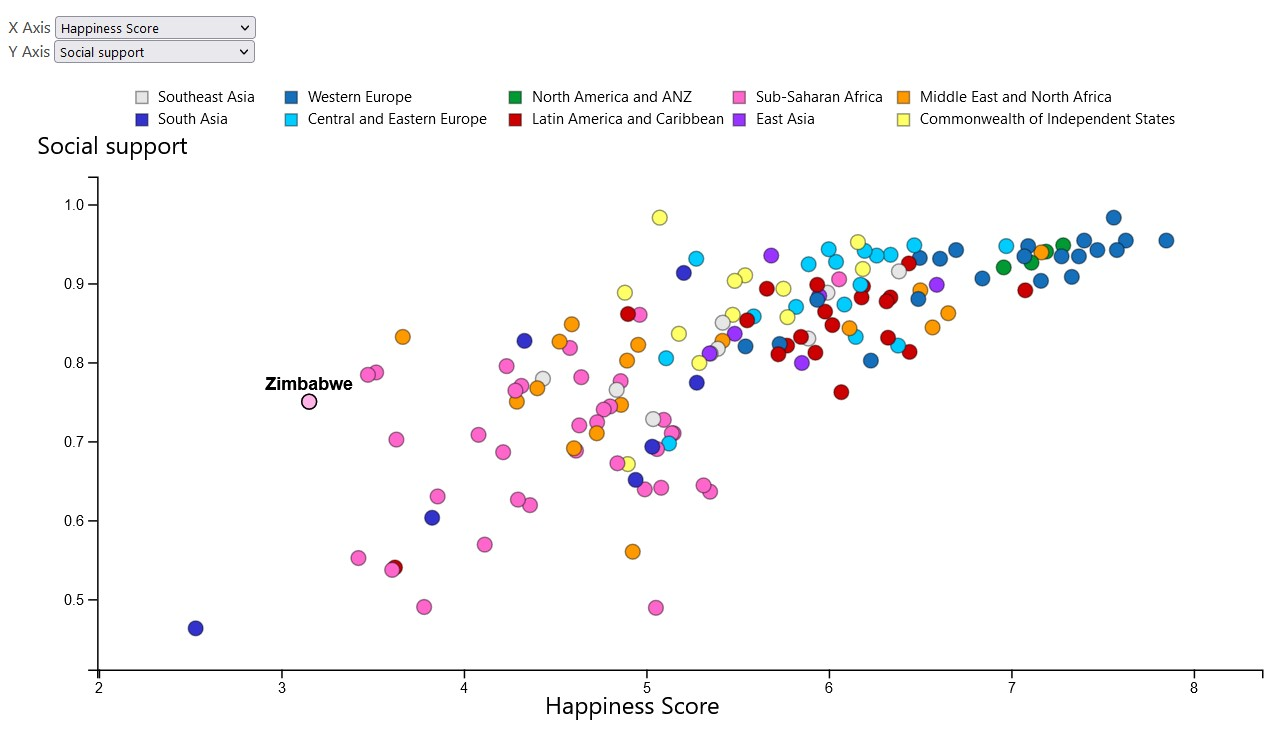
\includegraphics[width = \textwidth]{img/scatterplot.jpg}
 \caption{Scatterplot mit Bedienelementen}
 \label{fig:scatterplot}
\end{figure}
\vspace{0.5cm}

Der Scatterplot skaliert die jeweils angezeigten Größen dynamisch, sodass möglichst viel des verfügbaren Raumes mit Datenpunkten ausgefüllt ist. Dies hilft dabei Muster und einzelne Datenpunkte besser sichtbar zu machen. Die Daten bieten sich für diese Art der Visualisierung an. Es sind nicht zu viele Datenpunkte um den Plot unübersichtlich zu machen. Wie in Abbildung.\ref{fig:scatterplot} zu sehen gibt es nur wenige stark überlappende Punkte. Es sind gleichzeitig ausreichend Datenpunkte um Muster leicht zu identifizieren. Möchte man einen einzelnen Punkt identifizieren kann man mit dem Mauszeiger über diesem schweben, dann erscheint wie in Abbildung \ref{fig:scatterplot} der Landesname über dem Punkt. In diesem Beispiel ist es Zimbabwe. 


\subsubsection{Visualisierung 2: Polarplot}

Der Polarplot soll es ermöglichen alle Details über ein Land auf einen Blick sichtbar zu machen. Alle Dimensionen befinden sich auf im Kreis angeordneten Achsen. Diese sind dabei jeweils auf die verschieden Größen skaliert und mit Beschriftungen versehen. Das Maximum der jeweiligen Gruppe liegt dabei jeweils am Kreisrand. So lässt sich jeder Wert eines Landes schnell einordnen. \\

Der Happiness Score wird hier nicht innerhalb des Plots abgebildet. Er wird in Textform unter dem augewählten Land angezeigt, wie in Abbildung \ref{fig:polarplot} zu sehen. Der Polarplot ist vermutlich eine Darstellung die nicht jeder schoneinmal gesehen hat, allerdings ist die Strukur sehr einfach gehalten worden. Die visuelle Klarheit sollte es den Nutzer leicht machen die Daten schnell erfassen zu können. \\

\begin{figure}[h]
 \centering
 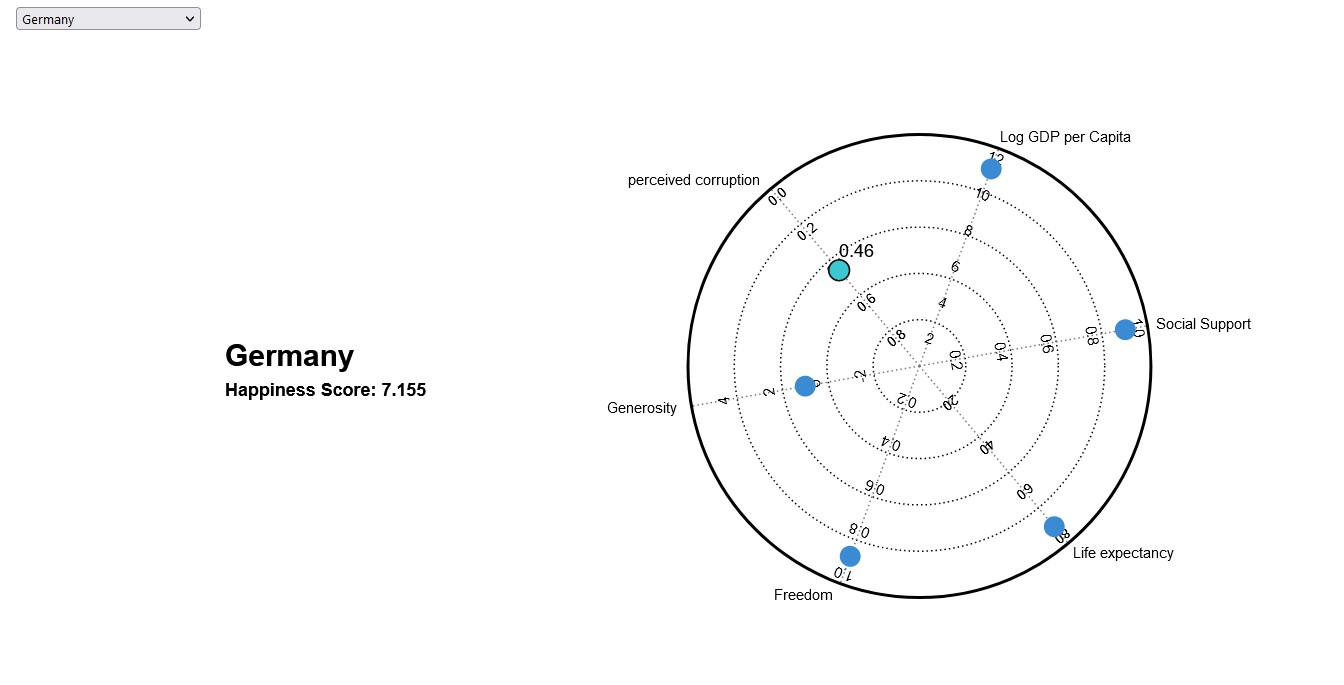
\includegraphics[width = \textwidth]{img/polarplot.jpg}
 \caption{Polarplot mit Bedienelementen}
 \label{fig:polarplot}
\end{figure}


Eine alternative Visualisierung währen hier Parallele Koordinaten gewesen. Diese sind auch in der Lage mehrere Dimensionen gleichzeitig darzustellen. Allerdings sind sie visuell möglicherweise etwas unklarer, die verbundenen Punkte auf den verschiedenen Achsen suggerieren eine Abfolge oder einen festen Zusammenhang dieser. Das ist für diesen Polarplot nicht der Fall. Ein Vorteil des Parallelplots ist Möglichkeit viele Instanzen, in diesem Fall Länder, gleichzeitig darzustellen. Je nach Einstellung der Verbindungslinien lässt sich dann auch eine Verteilung ausmachen. 

\subsubsection{Visualisierung 3: Zeitreihe}

Die letzte Darstellung verwendet den zweiten Datensatz aus dem World Happiness Report. Hier werden die historischen Daten dargestellt. Der Nutzer hat die Möglichkeit hier eine Größe zweier Länder zeitlich zu betrachten. Dies ermöglicht den Vergleich der Länder über einen Zeitraum von ca. 15 Jahren. Es lässt sich hier ein Eindruck darüber zu gewinnen wie sich die Größen in den verschiedenen Ländern mit der Zeit verändern. 

Hier gibt es kaum andere Möglichkeiten diese Zeitliche Entwicklung darzustellen. Möglicherweise hätte man die Jahreswerte auch mittels eines Balkendiagrammes für die jeweils ausgewählten Länder darstellen können. Allerdings wird hier der Zusammenhang, beziehungsweise die zeitliche Entwicklung nicht klar dargestellt. \\

\begin{figure}[h]
 \centering
 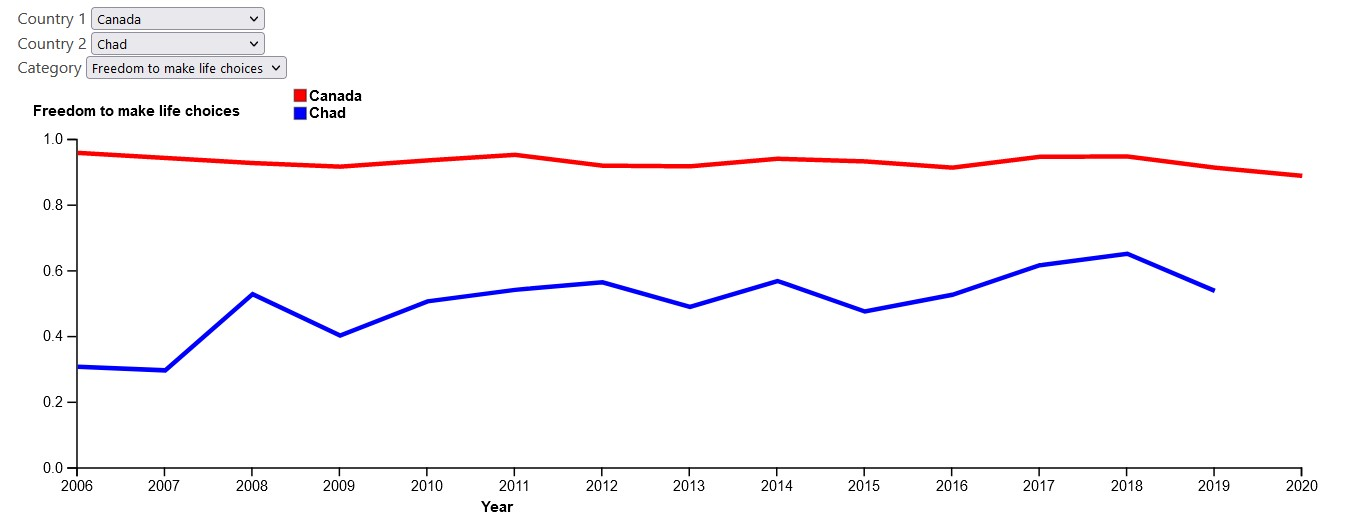
\includegraphics[width = \textwidth]{img/timeseries.jpg}
 \caption{Zeitreihe mit Bedienelementen}
 \label{fig:timeseries}
\end{figure}

Für diese Darstellung war die Wahl eines passenden Aspect Ratios entscheidend. Dieses hat großen Einfluss darauf wie deutlich Veränderungen zu sehen sind und wie vergleichbar sie untereinander sind. Hier wäre es möglich gewesen eine  Methode wie \textit{Banking to 45 degree} anzuwenden. Allerding wären die Ergebnisse für jedes paar von Ländern etwas unterschiedlich ausgefallen und somit eine Darstellung entstanden die immer ihre Größe ändert. Daher wurden einige Aspect Ratios ausprobiert und eines dann als Standard festgelegt.\\

Zu beachten ist bei dieser Darstellung, dass sie mit etwas unvollständigen Daten arbeitet. Die beiden vorherigen Darstellungen haben für jedes Land und jede Größe einen Wert. Hier fehlen bei einigen Länder Werte in einigen Jahren. Die fehlenden Jahre wurden hier durch das Zeichnen der Linien interpoliert. Dadurch haben alle Länder ununterbrochene Linien, sie starten und Enden aber in unterschiedlichen Jahren. Es wurde keine Extrapolation durchgeführt um Jahre zu ergänzen. Es sind hier auch zwei weitere Größen verfügbar welche im ersten Datensatz nicht enthalten sind. \textit{Positive Affect} und \textit{Negative Affect}. Sozusagen die Stimmung des jeweiligen Landes. Leider waren diese für die Durchschnitte nicht gegeben. Von einer nachträglichen Ergänzung wurde abgesehen. 

\subsection{Interaktion}

Der Scatterplot weist die meisten Interaktionsmöglichkeiten auf. Es lassen sich beide Achsen vom Nutzer anpassen um die dort angezeigten Größen zu verändern, dies passiert über die Dropdown Menüs über dem Plot. Bewegt ein Nutzer seinen Mauszeiger über einen Datenpunkt so wird der zugehörige Landesname angezeigt. Dies soll eine tiefere Auseinandersetzung mit den Daten ermöglichen. Ein nicht interaktiver Scatterplot würde diese Möglichkeit nicht bieten können. \\

Allerdings ist hier nicht nur die Information über den Landesnamen enthalten. Klickt der Nutzer auf den Datenpunkt werden die beiden anderen Plots angepasst. Der Polarplot wechselt auf das angeklickte Land. So lässt sich das Land im Detail mit allen zur Verfügung stehenden Größen betrachten. Die Zeitreihen Darstellung setzt das angeklickte Land als \textbf{Land 1} fest. Hier sind nun auch die historischen Daten schnell zugänglich. Diese Mechanik soll das Erforschen des Datensatzes intuitiver machen. Hier ist noch anzumerken, dass es ein paar wenige Länder gibt bei denen die erste Linie verschwinden wird. Diese Länder fehlen in den historischen Daten. Es wurde sich bewusst dazu entschieden hier auf eine fehlende Linie zu wechseln. So wird klar, dass für diesen Wert keine Daten bestehen. Andernfalls würde wohl auf einen Programmfehler geschlossen.\\

Auch mit dem Polarplot ist es möglich zu interagieren, durch hovern über den Datenpunkten wird hier der genaue Wert für den jeweiligen Punkt angezeigt. 
Mit dem links oben platzierten Dropdown lässt sich ein Land aussuchen, welches den Nutzer interessiert. Es handelt sich hier um insgesamt 149 Länder, was im Dropdown unübersichtlich wird. Allerdings ist es möglich das Dropdown zu durchsuchen sobald man es angeklickt hat. Um den Nutzer darauf aufmerksam zu machen ist hierzu ein Hinweis  am Beginn der Visualisierungsseite platziert. Für die Zeitreihe sind drei Dropdowns verfügbar es lassen sich zwei Länder aus den historischen Datensets aussuchen, wie auch beim Polarplot lassen sich die Dropdowns durchsuchen. Das dritte Dropdown Menü ist für die betrachtete Kategorie.

\section{Implementierung}
\subsection{Allgemeiner Aufbau}
Die Elm Applikation ist in vier verschiedene Dateien/Module aufgeteilt. \texttt{Main.elm} ist dabei die Datei in welcher die eigentliche Visualisierung kompiliert wird. 
Sie greift auf die Module \texttt{Displaydata.elm}, \texttt{Polarplot.elm} und \texttt{Timeseries.elm} zu. 
Dabei enthält \texttt{Displaydata.elm} die Datenverarbeitungs Funktionalität sowie die Funktionen für die erste Visualisierung, den Scatterplot. 
Die \texttt{Polarplot.elm} Datei enthält die Funktionen für den Polarplot 
und die \break \texttt{Timeseries.elm} jene für die Timeseries.  Zusätzlich besteht noch \texttt{My\_types.elm} Datei, dies enthält die definierten Typen welche von den Modulen geteilt werden. Sie sind ausgesondert um Importschleifen innerhalb der Module zu verhindern.\\

\begin{figure}[ht]
\centering
\begin{mdframed}[backgroundcolor=backcolour]
\begin{minted}[breaklines, linenos, tabsize=2]{Elm}

type Model 
  =  Failure
  | Loading
  | Loaded WorldHappData

type Msg
  = GotText (Result Http.Error String)
  | GotTsdata (Result Http.Error String)
  | Scatterplot_yaxis Int
  | Scatterplot_xaxis Int
  | Polarplot_country Int
  | Timeseries_1 Int
  | Timeseries_2 Int
  | Timeseries_cat Int
  | Click_Scat Int
  
\end{minted}
\end{mdframed}
    \caption{Typen Msg und Model mit denen die Visualisierung gesteuert wird}
    \label{fig:Msg_Model}
\end{figure}

In der \texttt{Main.elm} ist die Model View Update Struktur zu finden. 
Hier wird in der init Funktion der command fetchData aufgerufen welcher die erste HTTP Get anfrage an die Datenseite im Github Repository schickt. 
Wird diese erfolgreich abgerufen wird ein Model erstellt welches den Datentyp \textit{WorldHappData} hat. 
Hier werden sowohl die Daten für die Visualisierungen gespeichert, als auch die Einstellungen für diese. Da zu diesem Zeitpunkt erst einer von zwei Datensätzen geladen ist, wird für den zweiten zunächst ein leerer Default abgespeichert. \\

Diese Speicherung löst den zweiten command aus, fetchTsData, dieser stellt den zweiten HTTP get request, dieses Mal für die historischen Daten. Wenn auch diese geladen wurden, sind alle Daten für die Seite vorhanden. Im View wird nun die Visualisierung aufgerufen. Hierzu zählen einige Elemente aus dem Bulma Modul\cite{elm-bulma} welche Textboxen und Styling von HTML in Elm vereinfachen. Die Visualisierungen befinden sich alle in der viewHappiness Funktion. Diese nimmt die Daten und Einstellungen und generiert daraus die Visualisierungen. \\


Wie in  Abbildung.\ref{fig:Msg_Model} zu sehen gibt es zwei Msg Typen die jeweils einen Result HTTP erzeugen. Dies sind die beiden HTTP get Requests die wie vorher genannt zuerst ausgeführt werden. Die restlichen Typen sind die Messages welche die Visualisierungen aktualisiert wenn ein Nutzer mit ihnen interagiert. Dabei wird jeweils aus einem Dropdown ein Element auswählt welches die Msg auslöst und so ein Update erzwingt, hierbei wird ein Int mitgereicht welcher zu einer Änderung der Einstellungen der jeweiligen Visualisierung korrespondiert. Die Einstellung wird im WorldHappData Model aktualisiert. \\

\begin{figure}[ht]
\centering
\begin{mdframed}[backgroundcolor=backcolour]
\begin{minted}[breaklines, linenos, tabsize=2]{Elm}

type alias WorldHappData = 
    { data : List Country_2021,
      ts_data : List Ts_data,
      y_axis : String,
      x_axis : String,
      polar_country : String,
      line_1 : String,
      line_2 : String,
      ts_cat : String
    }
  
\end{minted}
\end{mdframed}
    \caption{WorldHappData, Datentyp des Models}
    \label{fig:Worldhapp}
\end{figure}

Hier in Abbildung.\ref{fig:Worldhapp} ist der definierte Datentype des Models abgebildet. Er enthält jegliche Zustände des Modells welche durch die \textit{Type Msg} in Abbildung.\ref{fig:Msg_Model} aktualisiert werden. \\

\newpage
\subsection{Scatterplot}

Der Scatterplot baut in großen Teilen auf die bereits in den Übungen verwendeten Elemente auf. Hier werden auch dynamisch skalierte Achsen und nach Klassen angepasste Punkte eingesetzt. Um die Ländergruppen identifizieren zu können wurde eine Legende über dem Scatterplot hinzugefügt, diese besteht aus Rechtecken aus dem Typed.Svg Modul und zugehörigem Text. Die Funktion selbst nimmt 6 Argumente entgegen. Zwei Stringlisten, das sind die Ländernamen für jeden Punkt und die Region zu welcher sie gehören. Zwei \texttt{List Float} welche die x und y Werte für die jeweilig ausgewählten Attribute enthalten und noch zwei String welche die zugehörigen x-Achsen und y-Achsen Labels enthalten. 

Diese 

\subsection{Präsentation der Visualisierungen}
Präsentieren sie die visuelle Abbildungen und Kodierungen der Daten und Interaktionsmöglichkeiten. 
Sie müssen  begründen, warum und wie gut ihre Designentscheidungen die erstellten Anforderungen erfüllen. 
Weiterhin müssen sie begründen, warum die gewählte visuelle Kodierung der Daten für das zulösenden Problem passend ist.
Typische Argumente würden hier auf Wahrnehmungsprinzipien und Theorie über Informationsvisualisierung verweisen. 
Die besten Begründungen diskutieren explizit die konkrete Auswahl der Visualisierungen im Kontext von mehreren verschiedenen Alternativen. 
Machen sie hier nicht den Fehler, einfach nur Visualisierung aus den vorgegebenen Bereichen zu diskutieren, weil das in der Regel nicht sinnvoll ist.
Wenn sie sich für einen Scatterplot entschieden haben, ist ein Zeitreihendiagramm in der Regel keine Alternative.
Diskutieren sie also nicht einfach Zeitreihendiagramme, weil sie in den Anforderungenen an das Projekt neben Scatterplots stehen, sondern suchen sie nach echten alternativen Visualisierungen, die zum Aufbau eines vergleichbaren mentalen Modells führen. 
Diskutieren sie die Expressivität und die Effektivität der einzelnen Visualisierungen. 

Die eben beschriebenen Präsentationen und Begründungen sollen für jede der drei folgenden Visualisierungen durchgeführt werden. 
\subsubsection{Visualisierung Eins}
\subsubsection{Visualisierung Zwei}
\subsubsection{Visualisierung Drei}

\subsection{Interaktion}
Die präsentierten Visualisierungstechniken müssen interaktiv zu einer Anwendung verknüpft werden.
Die Interaktion mit einer Visualisierung soll in den anderen Visualisierungen zu einer Änderung führen. 
Erklären sie die möglichen Interaktionen mit den einzelnen Visualisierungen und die möglichen Verknüpfungen zwischen ihnen. Begründen Sie warum die konkreten Interaktionen umgesetzt wurden und welche Zwecke für die Anwenderinnen mit ihnen unterstützt werden. Begründen sie ebenfalls warum sie andere Interaktionsmöglichkeiten nicht umgesetzt haben. Wenn sie keine der geforderten Interaktionen umsetzen, erhalten Sie im gesamten Projekt deutlichen Punktabzug. 

\section{Implementierung}
Beschreiben Sie die Implementierung ihrer Visualisierungsanwendung in Elm. Stellen die Gliederung ihres Quellcodes vor. Haben Sie verschiedene Elm-Module erstellt. Was war aufwändig umzusetzen, was ließ sich mit dem vorhanden Code aus den Übungen relativ einfach umsetzen? 

Wie sieht die Elm-Datenstruktur für das Model aus, in dem die verschiedenen Zustände der Interaktion gespeichert werden können.

\section{Anwendungsfälle}
Präsentieren sie für jede der drei Visualisierungen einen sinnvollen Anwendungsfall in dem ein bestimmter Fakt, ein Muster oder die Abwesenheit eines Musters visuell festgestellt wird. Begründen sie warum dieser Anwendungsfall wichtig für die Zielgruppe der Anwenderinnen ist. Diskutieren sie weiterhin, ob die oben beschriebene Information auch mit anderen Visualisierungstechniken hätte gefunden werden können. Falls dies möglich wäre, vergleichen sie die den Aufwand und die Schwierigkeiten ihres Ansatzes und der Alternativen. 
\subsection{Anwendung Visualisierung Eins}
\subsection{Anwendung Visualisierung Zwei}
\subsection{Anwendung Visualisierung Drei}

\section{Verwandte Arbeiten}
Führen sie eine kurze Literatursuche in der wissenschaftlichen Literatur zu Informationsvisualisierung und Visual Analytics nach ähnlichen Anwendungen durch. Diskutieren sie mindestens zwei Artikel. Stellen sie Gemeinsamkeiten und Unterschiede dar.

\section{Zusammenfassung und Ausblick}
Fassen sie die Beiträge ihre Visualisierungsanwendung zusammen. Wo bietet sie für die Personen der Zielgruppe einen echten Mehrwert.

Was wären mögliche sinnvolle Erweiterungen, entweder auf der Ebene der Visualisierungen und/oder auf der Datenebene?

\section*{Anhang: Git-Historie}

\printbibliography

\end{document}

